\section{Phase II Step 5: Smart-Contract Feasibility Scoring}
\label{sec:phase2_feasibility_scoring}

After completing C1--C4, the next step is to test whether the empirically useful metrics can also work inside
the DESTINO-aligned evidence model. This step applies the predefined smart-contract feasibility rubric from
Section~\ref{sec:feasibility_rubric_full}. The goal is not to move repository analysis on-chain. The intended
PoC architecture remains hybrid: metric extraction is performed off-chain from hash-pinned evidence, while the
contract stores compact values, provenance metadata, and evidence commitments.

This is a separate computation from C2, C3, and C4. Those criteria each score five criterion-specific dimensions
on a 0--10 scale. The feasibility pass scores ten smart-contract dimensions, D1--D10, on a 0--20 scale.

\subsection{Scoring protocol and artifacts}
\label{sec:feasibility_protocol_artifacts}

The feasibility pass has two layers. First, it combines the C1--C4 evidence into one metric-comparison table.
Second, it applies the ten-dimension feasibility rubric to each candidate. A metric is eligible for the final
PoC selection gate only if it is implemented in the current evidence base, is suitable as a reputation signal,
and does not trigger a feasibility exclusion condition.

\begin{table}[H]
\centering
\scriptsize
\renewcommand{\arraystretch}{1.08}
\begin{tabularx}{\textwidth}{p{5.6cm}rX}
\toprule
\textbf{Artifact} & \textbf{Rows} & \textbf{Role} \\
\midrule
\path{out/phase2_metric_comparison_all.csv} & 5 & Combined C1--C4 comparison scores and metric roles. \\
\path{out/feasibility_rubric_all.csv} & 10 & Fixed smart-contract feasibility dimensions. \\
\path{out/feasibility_scores_all.csv} & 50 & Per-metric, per-dimension feasibility scores and rationales. \\
\path{out/feasibility_summary_all.csv} & 5 & Metric-level feasibility totals, exclusions, and implementation stories. \\
\path{out/poc_candidate_decision_inputs_all.csv} & 5 & Combined empirical and feasibility inputs for the final selection gate. \\
\path{logs/feasibility_scoring_20260509.log} & 1 & Execution log for the feasibility scoring run. \\
\bottomrule
\end{tabularx}
\caption{Smart-contract feasibility scoring artifacts. Paths are relative to the Phase II analysis directory.}
\label{tab:feasibility_artifacts}
\end{table}

\subsection{Combined C1--C4 comparison}
\label{sec:combined_c1_c4_comparison}

The combined comparison keeps the role of each metric explicit. M1 receives strong stability and feasibility
scores, but it remains a context metric rather than a developer-reputation metric. M5 remains a design extension
because the current dataset does not contain issue or pull-request event streams. The implemented reputation
candidates are therefore M2, M3, and M4.

\begin{table}[H]
\centering
\scriptsize
\renewcommand{\arraystretch}{1.08}
\begin{tabularx}{\textwidth}{p{0.8cm}p{3.1cm}cccccX}
\toprule
\textbf{ID} & \textbf{Metric} & \textbf{C1} & \textbf{C2} & \textbf{C3} & \textbf{C4} & \textbf{Avg.} & \textbf{Role} \\
\midrule
M1 & Snapshot size & 10.0 & 8 & 5 & 7 & 7.50 & Context only; useful for normalization, not standalone reputation. \\
M2 & Churn & 4.0 & 8 & 7 & 7 & 6.50 & Eligible supporting candidate with volatility and quality caveats. \\
M3 & Activity cadence & 6.0 & 9 & 6 & 8 & 7.25 & Eligible continuity candidate with commit-splitting safeguards. \\
M4 & Ownership/concentration & 8.5 & 7 & 9 & 8 & 8.13 & Eligible reputation-oriented candidate with identity caveats. \\
M5 & Maintenance responsiveness & 0.0 & 6 & 3 & 4 & 3.25 & Design extension excluded from the current empirical decision. \\
\bottomrule
\end{tabularx}
\caption{Combined C1--C4 decision inputs. C1 is derived from primary high-volatility project counts; C2--C4 use the scored summaries from the previous sections.}
\label{tab:phase2_combined_comparison}
\end{table}

This table clarifies the empirical tradeoff. M4 has the strongest implemented reputation-oriented profile because
it combines better C1 stability than M2 and M3 with the strongest C3 gaming-resistance result and high C4
long-term suitability. M3 remains a strong alternative because it is easy to explain and compact over long histories,
but C3 showed that activity cadence is easier to manipulate. M2 remains useful evidence of effort, but the C1 result
shows that churn is too volatile to use alone.

\subsection{Feasibility results}
\label{sec:feasibility_results}

\begin{table}[H]
\centering
\scriptsize
\renewcommand{\arraystretch}{1.08}
\begin{tabularx}{\textwidth}{p{0.8cm}p{3.1cm}p{2.0cm}ccp{1.5cm}X}
\toprule
\textbf{ID} & \textbf{Metric} & \textbf{Role} & \textbf{Score} & \textbf{Band} & \textbf{Excl.} & \textbf{Interpretation} \\
\midrule
M1 & Snapshot size & Context only & 18/20 & High & None & Technically feasible, but not a standalone reputation metric. \\
M2 & Churn & Eligible & 16/20 & High & None & Feasible as a release-window aggregate with hash-pinned replay evidence. \\
M3 & Activity cadence & Eligible & 17/20 & High & None & Strong feasibility because cadence values are compact and release-window based. \\
M4 & Ownership/concentration & Eligible & 16/20 & High & None & Feasible in a hybrid model, with identity canonicalization kept explicit. \\
M5 & Responsiveness & Excluded & 10/20 & Medium & A; C & Not eligible because current evidence cannot replay or verify issue/PR events. \\
\bottomrule
\end{tabularx}
\caption{Smart-contract feasibility summary. Exclusion labels follow Section~\ref{sec:feasibility_rubric_full}.}
\label{tab:feasibility_summary}
\end{table}

\begin{figure}[H]
\centering
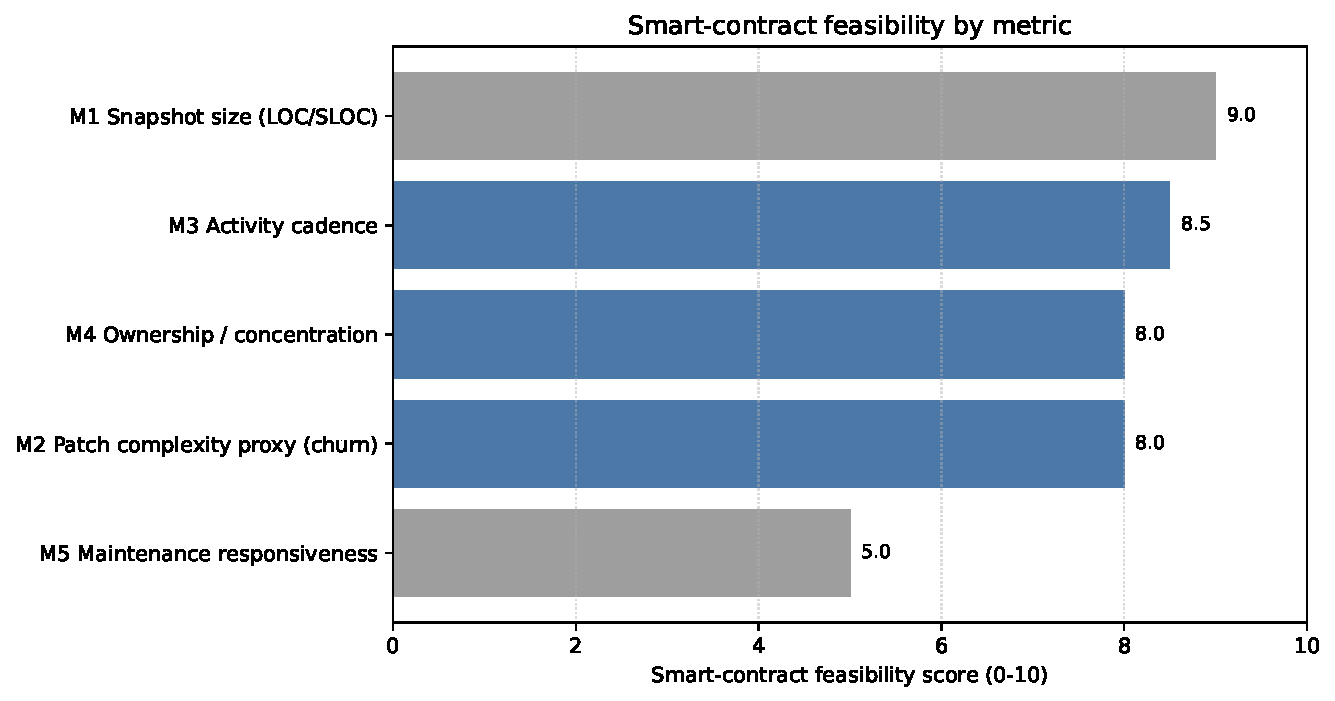
\includegraphics[width=0.90\textwidth]{figures/month3_feasibility/feasibility_scores.pdf}
\caption{Smart-contract feasibility scores on a 0--10 scale. Grey bars indicate metrics that are not eligible for the current PoC decision.}
\label{fig:feasibility_scores}
\end{figure}

The feasibility scores support the hybrid architecture defined earlier in the report. None of M2, M3, or M4 requires
the contract to traverse a repository or recompute a metric on-chain. Their feasible implementation story is to compute
the metric off-chain from frozen, hash-pinned evidence, then store a compact metric value and evidence hash on-chain.
The main differences are in storage shape and identity handling. M3 is the most compact eligible candidate. M4 is more
reputation-relevant, but requires careful handling of developer identity and fixed-point representation for shares or
concentration values.

\subsection{Final selection inputs}
\label{sec:final_selection_inputs}

The final decision-input table combines the C1--C4 average with the feasibility score. For ranking eligible metrics,
the current pass uses a transparent weighting: 60\% empirical comparison and 40\% smart-contract feasibility. This
weighting is not meant to hide the individual criteria; it is only a compact ordering tool after the separate scores
have been reported.

\begin{table}[H]
\centering
\scriptsize
\renewcommand{\arraystretch}{1.08}
\begin{tabularx}{\textwidth}{p{0.8cm}p{3.1cm}ccccX}
\toprule
\textbf{ID} & \textbf{Metric} & \textbf{C1--C4 avg.} & \textbf{Feas.} & \textbf{Combined} & \textbf{Rank} & \textbf{Selection status} \\
\midrule
M4 & Ownership/concentration & 8.13 & 8.0 & 8.08 & 1 & Preferred for the final selection gate. \\
M3 & Activity cadence & 7.25 & 8.5 & 7.75 & 2 & Eligible alternative. \\
M2 & Churn & 6.50 & 8.0 & 7.10 & 3 & Eligible alternative and supporting evidence. \\
M1 & Snapshot size & 7.50 & 9.0 & 8.10 & -- & Not selected as a standalone metric because it is context only. \\
M5 & Responsiveness & 3.25 & 5.0 & 3.95 & -- & Not selected because current evidence is absent and exclusions are triggered. \\
\bottomrule
\end{tabularx}
\caption{Final decision inputs before selecting the baseline PoC metric.}
\label{tab:poc_candidate_decision_inputs}
\end{table}

\begin{figure}[H]
\centering
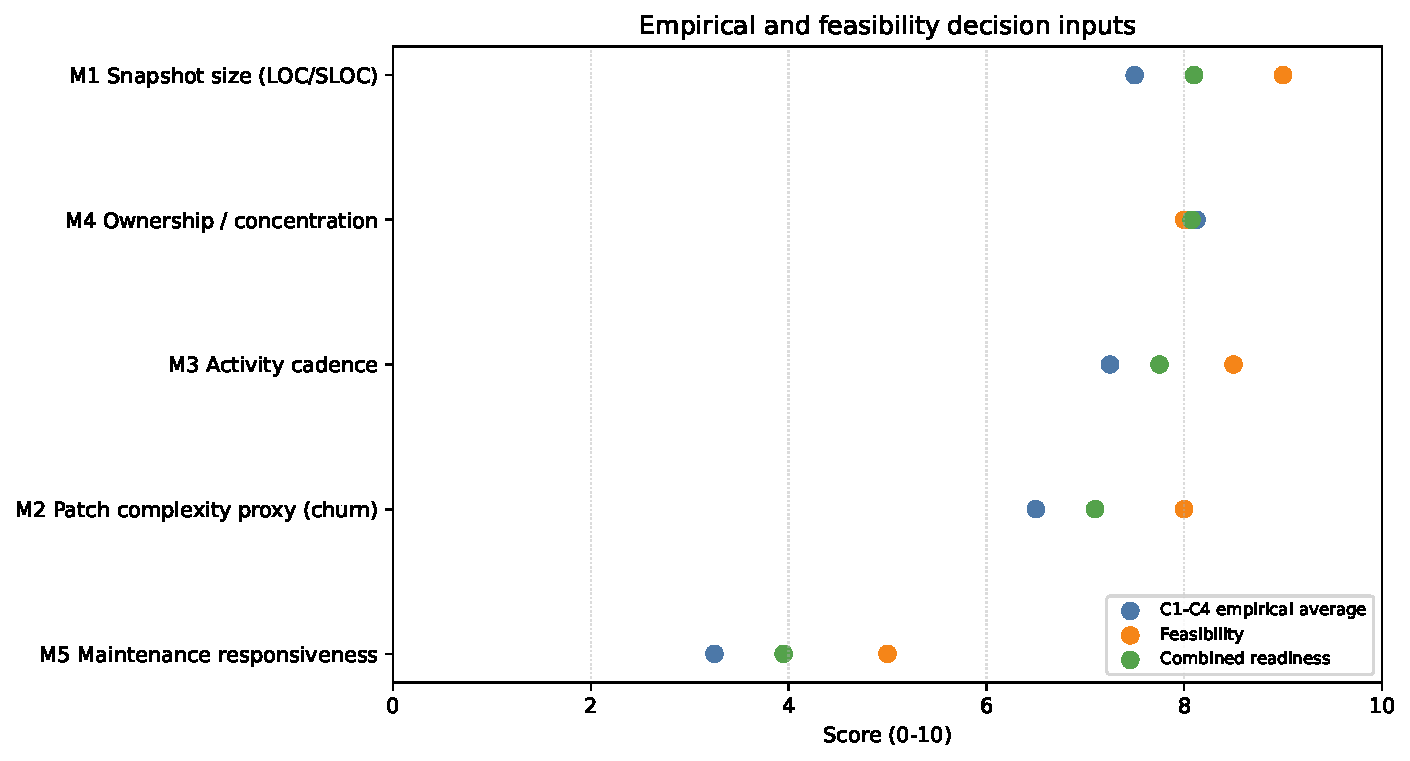
\includegraphics[width=0.92\textwidth]{figures/month3_feasibility/poc_candidate_readiness_scores.pdf}
\caption{Empirical, feasibility, and combined readiness scores used for the final selection gate.}
\label{fig:poc_candidate_readiness}
\end{figure}

The current evidence points to M4 ownership/concentration as the strongest eligible candidate for the final selection
gate. This does not mean that M3 and M2 are discarded. Instead, they should remain as supporting evidence and safeguards:
M3 helps interpret activity continuity, and M2 helps check whether ownership changes are backed by actual change effort.
M1 remains necessary for context and normalization. M5 remains future work.

The next step is to record the final metric-selection rationale and instantiate the selected metric in the
DESTINO-aligned PoC record shape.
